\documentclass[a4paper,12pt]{article}

\usepackage[a4paper,left=2.54cm,right=2.54cm,top=2.54cm,bottom=2.54cm]{geometry}

\usepackage[croatian]{babel}
\usepackage[utf8]{inputenc}
\usepackage{times}

\usepackage{amsmath} 
\usepackage{amssymb}

\usepackage{setspace}
\onehalfspacing

\usepackage{titlesec}
\titleformat{\section}{\fontsize{16pt}{20pt}\selectfont\bfseries}{\thesection.}{0.4cm}{}
\titleformat{\subsection}{\fontsize{14pt}{18pt}\selectfont\bfseries}{\thesubsection.}{0.4cm}{}
\setlength{\parskip}{10pt}

\titlespacing*{\section}{0pt}{0.5cm}{0pt}
\titlespacing*{\subsection}{0pt}{0.5cm}{0pt}

\usepackage{enumitem}
\setlist{topsep=3pt,itemsep=3pt}

\usepackage{graphicx,caption}

\usepackage[numbers]{natbib}
\setlength{\bibsep}{2pt}


\begin{document}

%%%%%%%%%%%%%%%%%%%%%%%%%%% NASLOVNICA %%%%%%%%%%%%%%%%%%%%%%%%%%%%%%%%%%%%%%%%%%%%%%%%%%%
\thispagestyle{empty}
\begin{center}
Sveučilište u Zagrebu\\
Fakultet organizacije i informatike
\end{center}
\vfill
\begin{center}
\Large Uvod u THREEjs
\end{center}
\vfill
\begin{flushright}
Tim: Karlo Jačmenjak \break
Antonio Kupčić \break
Josip Mojzeš \break
\end{flushright}
U Varaždinu, 2.1.2023. 

\newpage
\setcounter{page}{1}
%%%%%%%%%%%%%%%%%%%%%% KRAJ NASLOVNICE %%%%%%%%%%%%%%%%%%%%%%%%%%%%%%%%%%%%%%%%%%%%%%%%%%%

\section{Uvod}
\textbf{THREE.js} je JavaScript cross platform biblioteka i sučelje za programiranje aplikacija (API) koje se koristi za stvaranje i prikaz animirane 3D računalne grafike u web pregledniku pomoću WebGL-a. Izvorni kod THREE.js-a je otvorenog tipa.

%\begin{flushleft}
    Za početak rada u THREE.js prvo moramo dobiti WebGL kontekst, stvoriti novu scenu 
%\end{flushleft}


\begin{figure}[ht]
    \centering
    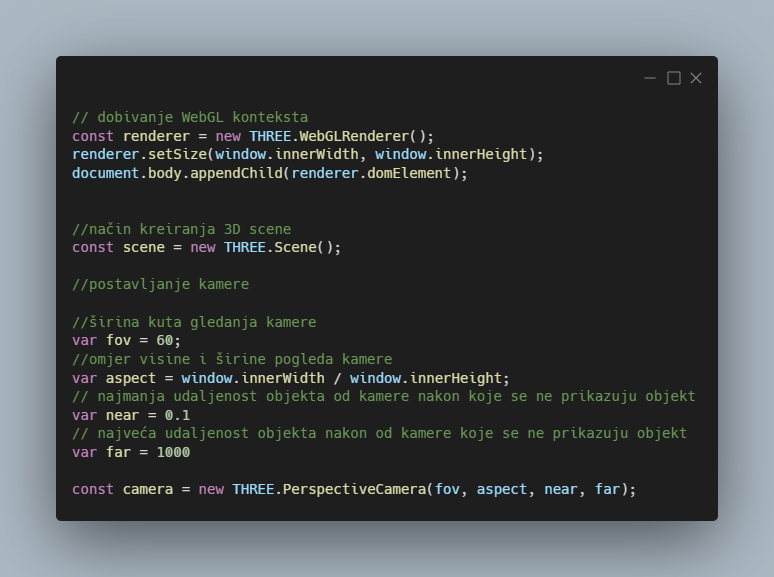
\includegraphics[scale=0.5]{image/zadatak1.png}
    \caption{Primjer koda za postavljanje kamere.}
\end{figure}


Dakle kao što vidimo na slici 3D scena se kreira na Three.Scene() funkcijom. Da bi smo postavili kameru trebamo koristiti četiri varijable, a to su 
varijabla \textit{fov} koja se koristi za širinu kuta gledanja, \textit{aspect} za omjer visine i širine pogleda pomoću ugrađenih objekata browsera, \textit{near} je 
varijabla koja se koristi za predstavljanje najmanje udaljenosti gdje se objekt ne prikazuje na kameri te varijabla \textit{far} koja je predstavljanje najveću 
udaljenost gdje se objekt ne prikazuje na kameri.
varijabla \textit{camera} služi tome da se prije navedene četiri varijable stave kao parametri u funkciju \texttt{PerspectiveCamera}.

\begin{figure}[ht]
    \centering
    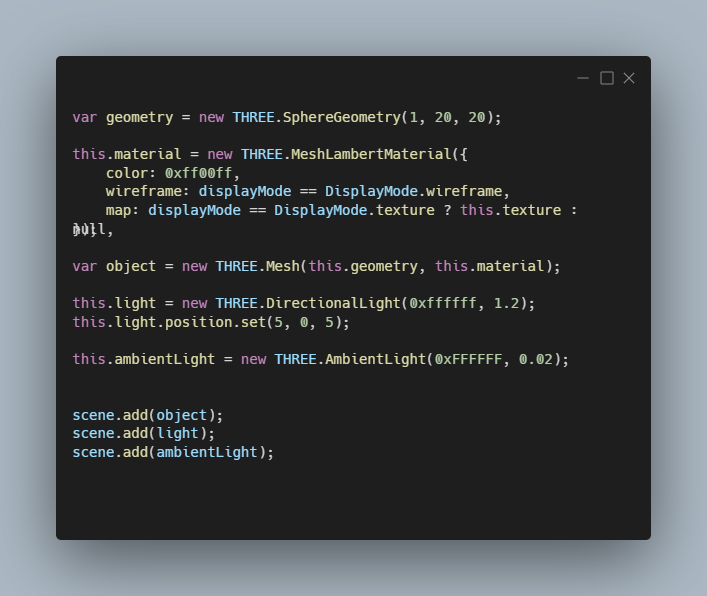
\includegraphics[scale=0.5]{image/zadatak1_objekti.png}
    \caption{Primjer koda za dodavanje objekta sceni te postavljanje svijetlosti i materijala.}
\end{figure}

\pagebreak
Da bi smo dodali objekt u scenu moramo napraviti varijablu \textit{object} koja je predstavlja fukciju \texttt{Mesh}. \texttt{Mesh} je funkcija koja poprima dva parametra, a to su materijal i 
vrstu geometrijskog tijela. U kodu na slici se radi o sferi pa se prvo mora stvoriti varijabla \textit{geometry} koja predstavlja funkciju \texttt{SphereGeometry} koja stvara sferu.
Drugi parametar funkcije \texttt{Mesh} je material. \textit{Material} je također varijabla koja predstavlja funkciju \texttt{MeshLamberMaterial} koja stvara materijal prema određenoj boji, 
prikazu i teksturi. Kada smo to sve napravili tada možemo pozvati \texttt{add} funkciju da stvorimo objekt. Svijetlo  se također postavlja sa \texttt{add}.
Varijabla \textit{light} predstavlja funkciju \texttt{DirectionalLight} koja stvara svijetlost te tu svijetlost postavljamo na neku poziciju. 

\begin{figure}[ht]
    \centering
    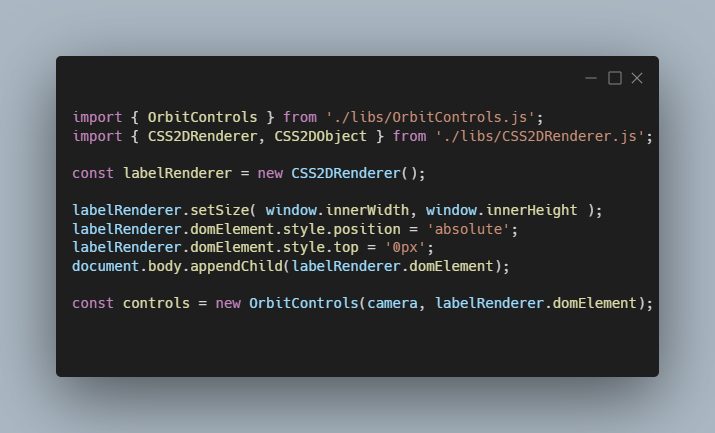
\includegraphics[scale=0.5]{image/zadatak1_kontrole.png}
    \caption{Primjer koda za interakciju miša i tastature s scenom.}
\end{figure}

\pagebreak
Interakcija preko miša i tastature se implementira se postiže sa objektima OrbitControls i renderer. Orbit controls omogućava da se kamera kreće oko modela,
a CSS2DRenderer prikazuje sve potrebne elemente modela.


\subsection{Podnaslov unutar uvoda}
Na primjer, definicija derivacije funkcije $f:I\to\mathbb{R}$ u točki $x_0\in I$ glasi
$$f'(x_0)=\lim_{\Delta x\to 0}{\frac{f(x_0+\Delta x)-f(x_0)}{\Delta x}}.$$
Ako želimo formulu automatski numerirati,
\begin{equation}
f'(x_0)=\lim_{\Delta x\to 0}{\frac{f(x_0+\Delta x)-f(x_0)}{\Delta x}},
\end{equation}
ili ju želimo označiti svojim simbolom
\begin{equation}
f'(x_0)=\lim_{\Delta x\to 0}{\frac{f(x_0+\Delta x)-f(x_0)}{\Delta x}}.\tag{$\clubsuit$}
\end{equation}

\newpage

\section{Aplet}
Cilj apleta je vizualno ilustrirati definiciju kardioide. Opišimo ukratko funkcioniranje apleta: BLA BLA BLA BLA
\begin{itemize}
\item Jedino što možete mijenjati u apletu je vrijednost parametra $t$ pomoću miša.
\item Za preciznije i sporije kretanje točke $T$, parametar $t$ mijenjajte pomoću strelica na tastaturi 
tako da najprije mišem kliknete na kružić od slidera, a nakon toga strelicama lijevo-desno mijenjate vrijednosti parametra $t$.
\item Pritiskom na tipku s trokutićem u donjem lijevom kutu možete pokrenuti animaciju tako da se parametar $t$ sam mijenja. Animaciju možete prekinuti pritiskom na tu istu tipku.
\item Prilikom kotrljanja kružnice točka $T$ ostavlja trag tako da se jasno vidi njezino geometrijsko mjesto točaka koje zovemo kardioida.
\item Ukoliko aplet ima fokus, pritiskom na \verb|CTRL+F| možete obrisati trag koji je ostavila točka $T$ prilikom kotrljanja kružnice.
\item Pritiskom na tipku u gornjem desnom kutu možete odmah vratiti aplet na početno zadane uvjete.
\end{itemize}
\LaTeX{} može ubaciti vanjsku sliku u svoj dokument. Slika pritom mora biti u odgovarajućem formatu i najjednostavnije je da se nalazi u tekućem
direktoriju \verb|tex| datoteke. Nadalje, \LaTeX{} ima dosta svojih fantastičnih paketa za crtanje slika kao što je \verb|tikz| paket.\par
\vspace*{5mm}
\begin{figure}[!h]
\centering

\caption{Kardioida u \texttt{GeoGebri}}
\end{figure}

\paragraph{Referenciranje na literaturu.} Prema literaturi \cite{Maric} vrijedi\,\ldots \ Prema literaturi \cite{geo} mora biti\,\ldots

\begin{thebibliography}{9}
\bibitem{Maric} An\dj elko Mari\'c, \emph{Vektori -- zbirka rije\v{s}enih zadataka}, Element, Zagreb, 1997.
\bibitem{geo} GeoGebra, \texttt{http://www.geogebra.org/cms/}, (9.3.2014.)
\end{thebibliography}

\end{document}